\chapter{Why Logic?}

\begin{goals}
\begin{itemize}
    \item Understand why logic emerged in the first place
    \item See how logic evolved from ``valid inference'' to something much broader
    \item Trace the journey from Aristotle to the four pillars of modern logic
\end{itemize}
\end{goals}

\section{What Logic Is Not}

Let's begin by clearing up a common confusion.

In everyday speech, ``logic'' means something like ``rational thinking'' or ``being reasonable.'' We say ``that's not logical'' when someone's argument doesn't make sense, or ``use your logic'' when we want someone to think carefully.

\textbf{Formal logic is not this.}

Formal logic is not \emph{only} about being smart, or thinking clearly, or avoiding fallacies in everyday reasoning---those may be corollaries, but they are not the core. The core is something much more specific, and in a way, much stranger.

At least, that was the \textbf{original} question:

\begin{quote}
Logic is the study of \textbf{implication}---the ``if... then...'' structure.

When can we say that one thing \emph{necessarily follows} from another? What does ``follows from'' even mean?
\end{quote}

This is where logic \emph{started}. But as we will see, the subject has traveled far from this origin---not abandoning it, but generalizing it beyond recognition. By the end of this chapter, ``implication'' will seem like just one special case of something much broader.

Think about it: implication is everywhere.
\begin{itemize}
    \item ``If it rains, the ground is wet'' (causation)
    \item ``If you are human, you are mortal'' (universal rule)
    \item ``If the program satisfies the precondition, it will satisfy the postcondition'' (specification)
    \item ``If these axioms hold, this theorem follows'' (proof)
\end{itemize}

All of these have the same \textbf{structure}: an antecedent (the ``if'' part) and a consequent (the ``then'' part). Logic studies this structure itself, abstracting away from what the antecedent and consequent actually say.

\section{Athens: Where It Began}

Why would anyone study such an abstract thing?

The answer lies in ancient Athens, where democracy meant public debate. Citizens argued in the assembly, in the courts, in the marketplace. To win an argument, you needed to \textbf{persuade}---and persuasion required making your reasoning visible and unchallengeable.

\begin{history}
The word ``logic'' comes from the Greek \emph{logos}, which means both ``word'' and ``reason.'' For the Greeks, language and thought were intimately connected. To speak well was to think well.
\end{history}

Imagine you're in a debate. Your opponent says something, you say something back. How do you \emph{win}? Not by shouting louder, but by showing that your conclusion \textbf{necessarily follows} from premises your opponent already accepts.

This is the birth of logic: the art of \textbf{valid argument}.

\begin{definition}[Validity, informally]
An argument is \textbf{valid} if the conclusion necessarily follows from the premises. That is, \emph{if} the premises are true, the conclusion \emph{must} be true.
\end{definition}

Note what validity does \emph{not} mean:
\begin{itemize}
    \item It does not mean the conclusion is true (the premises might be false)
    \item It does not mean the argument is convincing (it might be valid but irrelevant)
    \item It does not mean the argument is good (validity is just one criterion)
\end{itemize}

Validity is purely about the \textbf{structure} of the argument, not its content.

\section{Plato's World of Forms}

Before Aristotle systematized logic, his teacher Plato asked a deeper question: \textbf{what is truth?}

Plato observed that the physical world is messy and changeable. The circles we draw are imperfect, the chairs we sit on break and decay, the politicians we elect disappoint us. Yet we have a concept of a \emph{perfect} circle, an \emph{ideal} chair, a \emph{just} society.

Where do these perfect concepts come from?

\begin{history}
Plato's answer: there is a realm of \textbf{Forms} (or Ideas)---eternal, unchanging, perfect archetypes. The physical world is just a shadow of this realm. True knowledge is knowledge of the Forms, not of their imperfect shadows.
\end{history}

This sounds mystical, but it has a very practical implication for logic:

\begin{intuition}
Logical truths are not about this table or that chair. They are about the \emph{form} of arguments themselves. When we prove that ``if all A are B, and all B are C, then all A are C,'' we are not talking about any particular A, B, or C. We are talking about the \textbf{structure}.

In a sense, logic lives in Plato's realm of Forms.
\end{intuition}

\section{Aristotle's Syllogism}

Plato's student Aristotle was more practical. He wanted to \textbf{systematize} valid reasoning---to give rules that anyone could follow to check if an argument is valid.

The result was the \textbf{syllogism}, the first formal system in history.

\begin{example}[A syllogism]
\begin{inference}
All men are mortal. \quad (major premise)\\
Socrates is a man. \quad (minor premise)\\
\rule{5cm}{0.4pt}\\
Therefore, Socrates is mortal. \quad (conclusion)
\end{inference}
\end{example}

The key insight: the validity of this argument depends only on its \textbf{form}, not on what ``men,'' ``mortal,'' or ``Socrates'' mean. We can replace them with any terms:

\begin{inference}
All A are B.\\
S is an A.\\
\rule{4cm}{0.4pt}\\
Therefore, S is B.
\end{inference}

This \textbf{is} the syllogism. Aristotle catalogued all the valid forms and showed how to reduce complex arguments to combinations of these basic patterns.

\begin{history}[title={Where do ``Barbara'' and ``Celarent'' come from?}]
Medieval scholars invented a mnemonic system for the valid syllogisms.\footnote{The earliest known version is from William of Sherwood (13th century). See \href{https://medievallogic.wordpress.com/2017/11/16/syllogism-mnemonics/}{Medieval Logic \& Semantics}.}

First, they labeled the four types of propositions with vowels:
\begin{center}
\begin{tabular}{cl}
\textbf{A} & All S are P \quad (universal affirmative) --- from \emph{affirmo} \\
\textbf{E} & No S are P \quad (universal negative) --- from \emph{nego} \\
\textbf{I} & Some S are P \quad (particular affirmative) --- from \emph{affirmo} \\
\textbf{O} & Some S are not P \quad (particular negative) --- from \emph{nego}
\end{tabular}
\end{center}

Then each valid syllogism got a name whose vowels encode its structure:
\begin{itemize}
    \item \textbf{Barbara} (AAA): All M are P. All S are M. $\therefore$ All S are P.
    \item \textbf{Celarent} (EAE): No M are P. All S are M. $\therefore$ No S are P.
    \item \textbf{Darii} (AII): All M are P. Some S are M. $\therefore$ Some S are P.
    \item \textbf{Ferio} (EIO): No M are P. Some S are M. $\therefore$ Some S are not P.
\end{itemize}

Even the consonants had meaning: the first letter (B, C, D, F) indicated which first-figure syllogism a more complex form could be reduced to, and letters like `s' and `p' indicated specific reduction operations.

This is perhaps the first example of \textbf{encoding logic in notation}---a theme that will recur throughout this book.
\end{history}

\begin{keyinsight}
Aristotle's revolution: \textbf{form can be studied independently of content}.

This is the founding insight of all formal logic. Once you abstract away the content, you can study validity mechanically, without understanding what the argument is about.
\end{keyinsight}

\section{The Long Sleep}

After Aristotle, logic was considered essentially complete. Medieval scholars refined the syllogism, added some complications, debated edge cases---but the basic framework remained unchanged for nearly two thousand years.

Why?

Perhaps because syllogistic logic was \textbf{good enough} for philosophy and theology, which were the main intellectual activities of the time. When you're debating the nature of God or the essence of substances, the simple subject-predicate structure of syllogisms suffices.

But then something changed.

\section{Leibniz's Dream}

In the 17th century, Gottfried Wilhelm Leibniz---mathematician, philosopher, diplomat, and inventor of calculus---had a vision.

\begin{history}
Leibniz dreamed of a \emph{characteristica universalis}: a universal symbolic language that could express all human thought. And a \emph{calculus ratiocinator}: a mechanical method to compute the truth of any statement.

``When there are disputes among persons, we can simply say: let us calculate, without further ado, and see who is right.''
\end{history}

This was wildly ambitious. Leibniz never achieved it. But his dream planted a seed: \textbf{reasoning as calculation}.

If arguments could be reduced to symbols, and validity could be checked by mechanical rules, then reasoning could be---in principle---automated.

\section{Boole's Algebra}

Two centuries later, George Boole took the first real step toward Leibniz's dream.

\begin{history}[title={The Laws of Thought, 1854}]
Boole realized that the logical operations AND, OR, NOT could be treated as algebraic operations. Propositions became variables, connectives became operations, and logical reasoning became solving equations.
\end{history}

\begin{example}[Boolean algebra]
Let $p$ represent ``it is raining'' and $q$ represent ``the ground is wet.''

The basic operations are defined by their \textbf{truth tables}:

\begin{center}
\begin{tabular}{cc|cccc}
$p$ & $q$ & $\neg p$ & $p \land q$ & $p \lor q$ & $p \to q$ \\
\hline
T & T & F & T & T & T \\
T & F & F & F & T & F \\
F & T & T & F & T & T \\
F & F & T & F & F & T \\
\end{tabular}
\end{center}

\begin{itemize}
    \item $\neg p$ (NOT): true when $p$ is false
    \item $p \land q$ (AND): true when both are true
    \item $p \lor q$ (OR): true when at least one is true
    \item $p \to q$ (implication): false only when $p$ is true and $q$ is false
\end{itemize}

Boole showed these satisfy algebraic laws: $p \land q = q \land p$, $p \lor (q \land r) = (p \lor q) \land (p \lor r)$, and so on. Logic became calculation.
\end{example}

This was a breakthrough: logic became a branch of mathematics. But Boole's algebra could only express \textbf{propositional} logic---combinations of whole propositions. It couldn't look inside propositions to see their structure.

``All men are mortal'' is just a single symbol $p$ in Boolean algebra. The internal structure (``all,'' ``men,'' ``mortal'') is invisible.

\section{Frege's Revolution}

The real transformation came in 1879, when Gottlob Frege published a small book with a forbidding title: \emph{Begriffsschrift} (Concept-Script).

Frege wanted to show that mathematics could be derived from pure logic. To do this, he needed a logic far more powerful than Aristotle's syllogisms or Boole's algebra.

\begin{keyinsight}
Frege introduced:
\begin{enumerate}
    \item \textbf{Quantifiers}: $\forall x$ (``for all $x$'') and $\exists x$ (``there exists an $x$'')
    \item \textbf{Predicates and relations}: $P(x)$, $R(x, y)$ instead of ``$S$ is $P$''
    \item \textbf{Nested structure}: $\forall x \exists y \, R(x, y)$ means something different from $\exists y \forall x \, R(x, y)$
\end{enumerate}
\end{keyinsight}

Why these two quantifiers, $\forall$ and $\exists$? Why not ``most,'' ``exactly three,'' or ``infinitely many''?

\begin{intuition}
$\forall$ and $\exists$ are the \textbf{minimal pair}: they correspond to Aristotle's ``All'' and ``Some,'' and they are \textbf{duals}:
\[
\forall x \, \varphi \;\equiv\; \neg \exists x \, \neg \varphi
\]
``Everything has property $\varphi$'' means ``there is nothing without property $\varphi$.''

Some quantifiers can be built from these. For example, ``at least two things are $P$'' is:
\[
\exists x \, \exists y \, (x \neq y \land P(x) \land P(y))
\]
And ``exactly one thing is $P$'' is:
\[
\exists x \, (P(x) \land \forall y \, (P(y) \to y = x))
\]
But others---like ``most'' or ``infinitely many''---\emph{cannot} be expressed in first-order logic at all. This is a real limitation, and it drove later work on \textbf{generalized quantifiers}.

Notice the pattern: $\forall$ = ``for all individuals,'' $\exists$ = ``for some individual.'' Later, modal logic will use the same pattern: $\Box$ = ``in all worlds,'' $\Diamond$ = ``in some world.'' This is not a coincidence.
\end{intuition}

This is \textbf{first-order logic}, and it is vastly more expressive than anything before.

\begin{example}[Expressing ``all men are mortal'' in first-order logic]
\[
\forall x \, (\mathrm{Man}(x) \to \mathrm{Mortal}(x))
\]
Now the internal structure is visible. We can combine this with other statements, quantify over different variables, express complex relationships.
\end{example}

Frege's logic could express most of mathematics. This was the birth of \textbf{modern logic}.

\section{The Foundational Crisis}

Frege's dream was to derive all of mathematics from logic. In 1903, just as the second volume of his \emph{Grundgesetze} (Basic Laws) was going to press, he received a letter from a young British philosopher named Bertrand Russell.

Russell had found a contradiction.

\begin{history}[title={Russell's Paradox}]
Consider the set of all sets that do not contain themselves:
\[
R = \{ x \mid x \notin x \}
\]
Does $R$ contain itself?
\begin{itemize}
    \item If $R \in R$, then by definition $R \notin R$. Contradiction.
    \item If $R \notin R$, then by definition $R \in R$. Contradiction.
\end{itemize}
\end{history}

Frege's system was inconsistent. His life's work was undermined.

Russell, together with Alfred North Whitehead, spent a decade trying to fix the problem. Their \emph{Principia Mathematica} (1910--1913) introduced \textbf{type theory} to avoid the paradox. The book was massive, dense, and took hundreds of pages to prove that $1 + 1 = 2$.

\begin{intuition}
The crisis revealed something important: logic is powerful, but \textbf{dangerous}. The same expressive power that lets you talk about ``all sets'' also lets you construct paradoxes. The boundaries of logic needed careful study.
\end{intuition}

\section{The Four Pillars}

The crisis sparked a golden age of research. In the early 20th century, four branches of mathematical logic crystallized, each asking a fundamental question:

\begin{center}
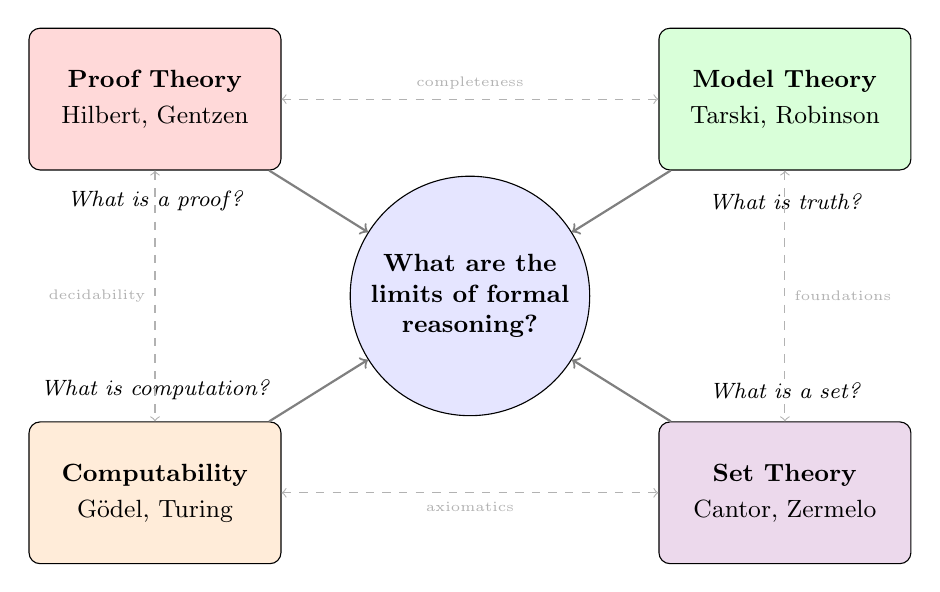
\begin{tikzpicture}[
    pillar/.style={draw, rounded corners, minimum width=3.2cm, minimum height=1.8cm, align=center, font=\small},
    question/.style={font=\footnotesize\itshape, text width=3cm, align=center},
    central/.style={draw, circle, minimum size=2.5cm, align=center, font=\small\bfseries, fill=blue!10},
]
    % Central question
    \node[central] (center) at (0,0) {What are the\\limits of formal\\reasoning?};

    % Four pillars
    \node[pillar, fill=red!15] (proof) at (-4, 2.5) {\textbf{Proof Theory}\\[2pt]Hilbert, Gentzen};
    \node[pillar, fill=green!15] (model) at (4, 2.5) {\textbf{Model Theory}\\[2pt]Tarski, Robinson};
    \node[pillar, fill=orange!15] (comp) at (-4, -2.5) {\textbf{Computability}\\[2pt]G\"odel, Turing};
    \node[pillar, fill=violet!15] (set) at (4, -2.5) {\textbf{Set Theory}\\[2pt]Cantor, Zermelo};

    % Questions
    \node[question] at (-4, 1.2) {What is a proof?};
    \node[question] at (4, 1.2) {What is truth?};
    \node[question] at (-4, -1.2) {What is computation?};
    \node[question] at (4, -1.2) {What is a set?};

    % Arrows
    \draw[->, thick, gray] (proof) -- (center);
    \draw[->, thick, gray] (model) -- (center);
    \draw[->, thick, gray] (comp) -- (center);
    \draw[->, thick, gray] (set) -- (center);

    % Connections between pillars
    \draw[<->, dashed, gray!60] (proof) -- node[above, font=\tiny] {completeness} (model);
    \draw[<->, dashed, gray!60] (proof) -- node[left, font=\tiny] {decidability} (comp);
    \draw[<->, dashed, gray!60] (model) -- node[right, font=\tiny] {foundations} (set);
    \draw[<->, dashed, gray!60] (comp) -- node[below, font=\tiny] {axiomatics} (set);
\end{tikzpicture}
\end{center}

These are not four unrelated subjects. They are four perspectives on the same question: \textbf{what are the limits and possibilities of formal reasoning?} The dashed lines show how deeply interconnected they are---completeness theorems link proof theory and model theory, decidability connects proofs to computation, and set theory provides the foundational language for all.

\subsection{Proof Theory}

David Hilbert launched a program: formalize all of mathematics, and prove that the formalization is consistent (free of contradictions).

Gerhard Gentzen developed \textbf{natural deduction} and the \textbf{sequent calculus}---ways of studying proofs as mathematical objects themselves. What is the structure of a proof? Can proofs be simplified? Transformed?

\subsection{Model Theory}

Alfred Tarski asked: what does it mean for a sentence to be \textbf{true}?

His answer: truth is a relationship between sentences (syntax) and structures (semantics). A sentence is true \emph{in a model}. Model theory studies this relationship: which sentences have models? How do models relate to each other? What can be expressed?

\subsection{Computability Theory}

Kurt G\"odel, Alonzo Church, and Alan Turing independently discovered the boundaries of computation.

G\"odel's incompleteness theorems (1931) showed that Hilbert's program was impossible: any sufficiently powerful consistent system contains true statements that cannot be proved.

Church and Turing (1936) defined what ``computable'' means, and showed that some problems (like the halting problem) are \textbf{undecidable}---no algorithm can solve them.

\subsection{Set Theory}

Georg Cantor had discovered that infinity comes in different sizes. But his naive set theory led to paradoxes.

Zermelo, Fraenkel, and others developed axiomatic set theory (ZFC), carefully restricting which sets can be formed. Paul Cohen later showed that some questions (like the continuum hypothesis) are \textbf{independent}---neither provable nor disprovable from the axioms.

\section{The Core Insight}

Beneath these four branches lies a single theme:

\begin{keyinsight}
Logic studies \textbf{the invariance of forms}.

What properties of a structure are preserved under what transformations?
\begin{itemize}
    \item Valid inference preserves truth.
    \item Bisimulation preserves modal properties.
    \item Computable functions preserve finiteness of description.
    \item Homomorphisms preserve algebraic structure.
\end{itemize}
The content changes, but something essential remains unchanged. Logic is the study of that ``something.''
\end{keyinsight}

This is why logic became useful to so many fields:

\begin{itemize}
    \item \textbf{Philosophers} needed it to analyze concepts precisely
    \item \textbf{Mathematicians} needed it to establish foundations
    \item \textbf{Linguists} needed it to describe the structure of language
    \item \textbf{Computer scientists} needed it to specify and verify programs
\end{itemize}

They all needed the same thing: a formal language to express structure, and rules to reason about structure while preserving essential properties.

\section{A Question for the Future}

We have traced logic from Athenian debates to the four pillars of modern mathematical logic. But this is not the end of the story.

A question lingers: \textbf{can we study ``invariance'' itself as a mathematical object?}

The four pillars use set theory as their common language. But sets are about \emph{membership} (what elements belong to what collections). Is there a language that directly talks about \emph{structure} and \emph{what is preserved under transformations}?

The answer is yes. It is called \textbf{category theory}, and it will transform how we think about logic.

But that is for the next chapter.

\begin{summary}
\begin{itemize}
    \item Logic is not ``being rational''---it \emph{began} as the study of valid inference, but has evolved far beyond
    \item Aristotle's syllogism: form can be studied independently of content
    \item Frege's revolution: quantifiers, predicates, and the ambition to ground all mathematics
    \item The foundational crisis led to four pillars: proof theory, model theory, computability, set theory
    \item The core insight: logic studies \textbf{the invariance of forms}
    \item This is why diverse fields all need logic---not for ``reasoning,'' but for describing structured systems
    \item Next: how logic became a \emph{language} for describing systems, not just a tool for checking arguments
\end{itemize}
\end{summary}
